
\section{Distribuciones de muestreo}

Esta secci\'on agrupa las herramientas t\'ecnicas que sustentan las distribuciones
muestrales. Las distribuciones que aqu\'i se estudian (Z, t, $\chi^2$, F) son la
columna vertebral de la inferencia estad\'istica cl\'asica y aparecen de manera
recurrente en problemas de ciencia de datos.


\subsection{Transformaci\'on de variables aleatorias}

Una pregunta frecuente en estad\'istica es: si $X$ tiene una distribuci\'on conocida
y definimos $Y = g(X)$ para alguna funci\'on $g$, ¿cu\'al es la distribuci\'on de $Y$?

\subsubsection{Transformaci\'on lineal}

\begin{teorema}[Transformaci\'on af\'in]
Si $X$ es una variable aleatoria con media $\mu_X$ y varianza $\sigma_X^2$, y
$Y = aX + b$ con $a \neq 0$, entonces
\begin{align}
 \label{eq:3.2.1}
 \mu_Y &= a\mu_X + b, \\
 \label{eq:3.2.2}
 \sigma_Y^2 &= a^2\sigma_X^2.
\end{align}
Adem\'as, si $X$ tiene funci\'on de distribuci\'on $F_X$, entonces
$F_Y(y) = F_X\!\left(\frac{y-b}{a}\right)$.
\end{teorema}

\begin{ejemplo}
 \label{exmp:3.2.1}
Si $X \sim N(\mu, \sigma^2)$ y $Y = aX + b$ con $a \neq 0$, entonces
$Y \sim N(a\mu + b, a^2\sigma^2)$. Esta es la \emph{propiedad de reproductividad}
de la distribuci\'on normal bajo transformaciones lineales.
\end{ejemplo}

\subsubsection{Teorema de cambio de variable}

Para transformaciones m\'as generales, necesitamos el siguiente resultado.

\begin{teorema}[Cambio de variable, caso mon\'otono]
Sean $X$ una variable aleatoria continua con densidad $f_X$, y $g$ una funci\'on
estrictamente mon\'otona y diferenciable. Si $Y = g(X)$ y $g^{-1}$ denota la inversa
de $g$, entonces la densidad de $Y$ es
\begin{align}
 \label{eq:3.2.3}
 f_Y(y) = f_X\!\left(g^{-1}(y)\right) \cdot \left|\frac{d}{dy}\,g^{-1}(y)\right|,
\end{align}
para todo $y$ en el rango de $g$.
\end{teorema}

\begin{proof}
Supongamos $g$ creciente. Para $y$ en el rango de $g$,
\begin{align}
 F_Y(y) = P(Y \leq y) = P(g(X) \leq y) = P(X \leq g^{-1}(y)) = F_X(g^{-1}(y)).
\end{align}
Derivando y aplicando la regla de la cadena,
\begin{align}
 f_Y(y) = \frac{d}{dy} F_X(g^{-1}(y)) = f_X(g^{-1}(y)) \cdot \frac{d}{dy} g^{-1}(y).
\end{align}
El caso $g$ decreciente es an\'alogo, tomando valor absoluto.
\end{proof}

\begin{observacion}[Forma alternativa]
Si escribimos $x = g^{-1}(y)$ y denotamos $J(y) = \frac{dx}{dy}$ el Jacobiano de la
transformaci\'on inversa, la f\'ormula se reescribe como
\begin{align}
 \label{eq:3.2.4}
 f_Y(y) = f_X(x)\,|J(y)|, \quad \text{donde } x = g^{-1}(y).
\end{align}
En dimensi\'on superior, $|J(y)|$ es el valor absoluto del determinante Jacobiano.
\end{observacion}

\begin{ejemplo}
 \label{exmp:3.2.2}
Sea $X \sim \text{Exp}(1)$ con densidad $f_X(x) = e^{-x}$ para $x > 0$. Encuentre la
distribuci\'on de $Y = e^X$.
\end{ejemplo}

\begin{solucion}
La transformaci\'on $g(x) = e^x$ es estrictamente creciente de $(0, \infty)$ a
$(1, \infty)$, con inversa $g^{-1}(y) = \ln y$. Adem\'as, $\frac{d}{dy}\ln y = 1/y$.

Por el teorema de cambio de variable, para $y > 1$:
\begin{align}
 f_Y(y) = f_X(\ln y) \cdot \frac{1}{y} = e^{-\ln y} \cdot \frac{1}{y} = \frac{1}{y} \cdot \frac{1}{y} = \frac{1}{y^2}.
\end{align}

Por lo tanto, $Y$ tiene densidad $f_Y(y) = 1/y^2$ para $y > 1$ (una distribuci\'on
de Pareto con par\'ametro $\alpha = 1$).
\end{solucion}

\begin{ejemplo}
 \label{exmp:3.2.3}
Sea $X \sim N(\mu, \sigma^2)$. Encuentre la distribuci\'on de $Y = e^X$ (la
distribuci\'on \emph{log-normal}).
\end{ejemplo}

\begin{solucion}
La transformaci\'on $g(x) = e^x$ es creciente, con inversa $g^{-1}(y) = \ln y$.
La densidad de $X$ es
\begin{align}
 f_X(x) = \frac{1}{\sigma\sqrt{2\pi}}\,\exp\!\left(-\frac{(x-\mu)^2}{2\sigma^2}\right).
\end{align}

Aplicando el teorema, para $y > 0$:
\begin{align}
 f_Y(y) &= f_X(\ln y) \cdot \frac{1}{y} \\
 &= \frac{1}{\sigma\sqrt{2\pi}}\,\exp\!\left(-\frac{(\ln y - \mu)^2}{2\sigma^2}\right) \cdot \frac{1}{y}.
\end{align}

Por lo tanto, $Y$ sigue una distribuci\'on log-normal $LN(\mu, \sigma^2)$.
\end{solucion}

\begin{ejemplo}
 \label{exmp:3.2.4}
Sea $X \sim U(0, 2\pi)$ uniforme. Encuentre la distribuci\'on de $Y = \sin(X)$ (caso
no mon\'otono).
\end{ejemplo}

\begin{solucion}
La funci\'on $g(x) = \sin x$ no es mon\'otona en $(0, 2\pi)$: alcanza el m\'aximo
$1$ en $x = \pi/2$ y el m\'inimo $-1$ en $x = 3\pi/2$. Cada valor $y \in (-1, 1)$
tiene dos preim\'agenes: $x_1 = \arcsin y$ y $x_2 = \pi - \arcsin y$.

Usando la f\'ormula para el caso no mon\'otono,
\begin{align}
 f_Y(y) &= \sum_{x: \sin x = y} f_X(x) \cdot \left|\frac{dx}{dy}\right| \\
 &= \frac{1}{2\pi}\cdot\frac{1}{\sqrt{1-y^2}} + \frac{1}{2\pi}\cdot\frac{1}{\sqrt{1-y^2}} \\
 &= \frac{1}{\pi\sqrt{1-y^2}}, \quad y \in (-1, 1).
\end{align}

Esta es la densidad del \emph{arcoseno}, que aparece en el \emph{camino aleatorio}.
\end{solucion}

\subsubsection{Transformaciones comunes}

\begin{observacion}
Las siguientes transformaciones son \'utiles para \emph{normalizar} datos o
estabilizar varianzas:
\begin{itemize}
 \item $Y = \ln X$: comprime valores grandes, expande valores cercanos a $0$.
 \item $Y = \sqrt{X}$: suaviza la asimetr\'ia de conteos.
 \item $Y = X^{1/3}$: alternativa a la ra\'iz cuadrada para datos con asimetr\'ia
 pronunciada.
 \item \emph{Box-Cox}: $Y = (X^\lambda - 1)/\lambda$ para $\lambda \neq 0$;
 $Y = \ln X$ para $\lambda = 0$. Optimiza la normalidad.
\end{itemize}
\end{observacion}

[fragile, allowframebreaks]{transformacionesVariables.py}
 \begin{verbatim}
import numpy as np
import matplotlib.pyplot as plt
from scipy import stats

# Ejemplo: distribuci\'on log-normal
np.random.seed(0)
mu, sigma = 0, 0.5
X = np.random.normal(mu, sigma, size=10000)
Y = np.exp(X)  # transformaci\'on

fig, axes = plt.subplots(1, 2, figsize=(12, 4))
axes[0].hist(X, bins=50, density=True, alpha=0.7, color='steelblue')
x_norm = np.linspace(-3, 3, 100)
axes[0].plot(x_norm, stats.norm.pdf(x_norm, mu, sigma), 'r-', lw=2)
axes[0].set_title('X ~ N(0, 0.5) (normal)')
axes[0].set_xlabel('x')

axes[1].hist(Y, bins=50, density=True, alpha=0.7, color='coral')
y_grid = np.linspace(0.01, 5, 100)
lognorm_pdf = stats.lognorm.pdf(y_grid, s=sigma, scale=np.exp(mu))
axes[1].plot(y_grid, lognorm_pdf, 'r-', lw=2)
axes[1].set_title('Y = exp(X) (log-normal)')
axes[1].set_xlabel('y')

plt.tight_layout()
plt.savefig('pe/transformaciones.png', dpi=100, bbox_inches='tight')
plt.show()

# Transformaci\'on Box-Cox
from scipy.stats import boxcox
datos = np.random.exponential(scale=2, size=1000)
datos_transformados, lambda_opt = boxcox(datos)
print(f"Lambda \'optimo: {lambda_opt:.3f}")
##Lambda \'optimo: 0.279
 \end{verbatim}

\begin{figure}
 \centering
 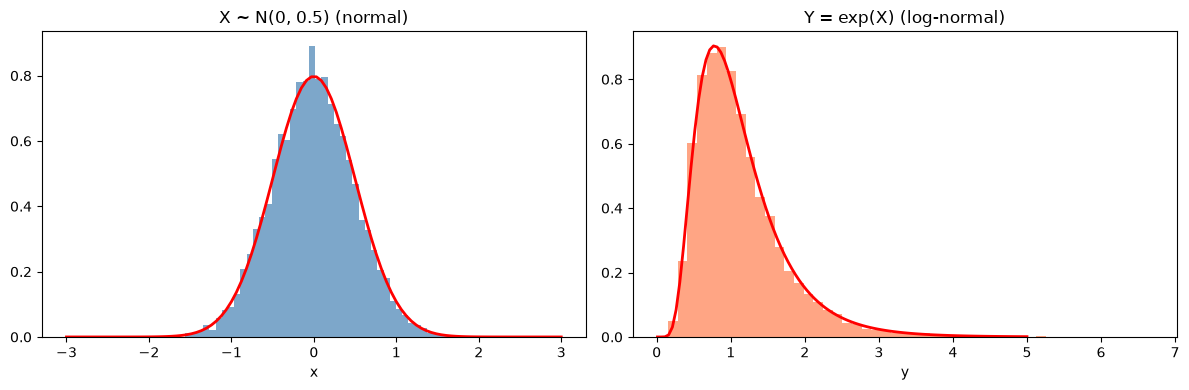
\includegraphics[height=7cm,keepaspectratio=true]{./pe/transformaciones.png}
 % transformaciones.png: 0x0 pixel, 300dpi, 0.00x0.00 cm, bb=
 \caption{Transformaci\'on exponencial: de normal a log-normal.}
 \label{fig:3.2.1}
\end{figure}



\subsection{Distribuciones de funciones de variables aleatorias}

Esta subsecci\'on generaliza los resultados anteriores al caso en que $Y$ es una
funci\'on (no necesariamente mon\'otona) de $X$ o de varias variables.

\subsubsection{Caso de una variable}

Cuando $g$ no es mon\'otona, hay que considerar todas las preim\'agenes de cada
valor $y$. La f\'ormula general es
\begin{align}
 \label{eq:3.2.5}
 f_Y(y) = \sum_{x \in g^{-1}(y)} f_X(x) \cdot \left|\frac{dx}{dy}\right|
 = \sum_{x: g(x) = y} \frac{f_X(x)}{|g'(x)|}.
\end{align}

\begin{observacion}
La condici\'on $|g'(x)| \neq 0$ en cada $x \in g^{-1}(y)$ garantiza que la
transformaci\'on es localmente invertible en cada preimagen.
\end{observacion}

\subsubsection{Caso de varias variables}

Si $(X_1, \ldots, X_n)$ tiene densidad conjunta $f_{X_1, \ldots, X_n}$ y
$Y = g(X_1, \ldots, X_n)$, la densidad de $Y$ se obtiene integrando la densidad
conjunta sobre el conjunto de nivel $g(x_1, \ldots, x_n) = y$:
\begin{align}
 \label{eq:3.2.6}
 f_Y(y) = \int \cdots \int_{g(x_1, \ldots, x_n) = y} f_{X_1, \ldots, X_n}(x_1, \ldots, x_n)
 \cdot \frac{dS}{|\nabla g|},
\end{align}
donde $dS$ es el elemento de \'area sobre la superficie de nivel y $\nabla g$ es
el gradiente de $g$.
\end{observacion}

\begin{ejemplo}
 \label{exmp:3.2.5}
Si $X_1, X_2 \sim \text{Exp}(1)$ son independientes, encuentre la distribuci\'on de
$Y = X_1 + X_2$.
\end{ejemplo}

\begin{solucion}
La funci\'on de densidad conjunta es $f(x_1, x_2) = e^{-(x_1+x_2)}$ para
$x_1, x_2 > 0$. La suma $Y = X_1 + X_2$ se obtiene integrando sobre la l\'inea
$x_1 + x_2 = y$:
\begin{align}
 f_Y(y) &= \int_0^y e^{-(x_1 + (y-x_1))}\,dx_1 = \int_0^y e^{-y}\,dx_1 = y\,e^{-y}, \quad y > 0.
\end{align}

Esta es la densidad Erlang con par\'ametro de forma $2$, o equivalentemente
$\text{Gamma}(2, 1)$. Generalizando, la suma de $n$ exponenciales iid es
$\text{Gamma}(n, 1)$ (ver secci\'on 2.11).
\end{solucion}



\subsection{Distribuciones muestrales de medias}

La distribuci\'on muestral de la media es fundamental para la inferencia estad\'istica.
Su tratamiento detallado se realiza en la secci\'on \ref{sec:3.4}; aqu\'i resumimos
los resultados principales.

Si $X_1, X_2, \ldots, X_n$ son variables aleatorias independientes e id\'enticamente
distribuidas (iid) con media $\mu$ y varianza $\sigma^2$, y $\bar{X} = \frac{1}{n}\sum X_i$,
entonces
\begin{align}
 \label{eq:3.2.7}
 E(\bar{X}) &= \mu, \\
 \label{eq:3.2.8}
 \text{Var}(\bar{X}) &= \frac{\sigma^2}{n}, \\
 \label{eq:3.2.9}
 \text{DE}(\bar{X}) &= \frac{\sigma}{\sqrt{n}}.
\end{align}

Adem\'as, por el Teorema del L\'imite Central, cuando $n$ es suficientemente grande,
\begin{align}
 \label{eq:3.2.10}
 \frac{\bar{X} - \mu}{\sigma/\sqrt{n}} \xrightarrow{d} N(0,1).
\end{align}

\begin{observacion}
La distribuci\'on exacta de $\bar{X}$ es \emph{normal} si la poblaci\'on original es
normal, y aproximadamente normal para $n$ grande en otros casos. Esta diferencia es
crucial: en el primer caso hablamos de $Z$ exacto; en el segundo, de $Z$ aproximado.
\end{observacion}



\subsection{Distribuci\'on $\chi^2$ (chi-cuadrada)}

La distribuci\'on $\chi^2$ aparece al sumar cuadrados de normales est\'andar. Su
tratamiento detallado se realiza en la secci\'on \ref{sec:3.9}; aqu\'i presentamos
los resultados esenciales.

\begin{definicion}[Distribuci\'on $\chi^2$]
Sean $Z_1, Z_2, \ldots, Z_\nu$ variables aleatorias independientes con $Z_i \sim N(0,1)$.
La variable aleatoria
\begin{align}
 \label{eq:3.2.11}
 \chi^2_\nu = \sum_{i=1}^\nu Z_i^2
\end{align}
sigue una distribuci\'on \emph{chi-cuadrada} con $\nu$ grados de libertad.
\end{definicion}

{Propiedades}
\begin{itemize}
 \item Media: $E(\chi^2_\nu) = \nu$.
 \item Varianza: $\text{Var}(\chi^2_\nu) = 2\nu$.
 \item Como caso particular de la familia gamma (secci\'on 2.11),
 $\chi^2_\nu = \text{Gamma}\!\left(\frac{\nu}{2}, 2\right)$.
 \item Reproductividad: si $\chi^2_{\nu_1}$ y $\chi^2_{\nu_2}$ son independientes,
 $\chi^2_{\nu_1} + \chi^2_{\nu_2} \sim \chi^2_{\nu_1 + \nu_2}$.
\end{itemize}

\begin{observacion}
La distribuci\'on $\chi^2$ surge naturalmente al estimar la varianza de una poblaci\'on
normal. Si $X_1, \ldots, X_n$ son normales iid y $S^2$ es la varianza muestral,
entonces
\begin{align}
 \frac{(n-1)S^2}{\sigma^2} \sim \chi^2_{n-1}.
\end{align}
Este resultado es la base de los intervalos de confianza para $\sigma^2$ y de la
prueba chi-cuadrada de bondad de ajuste.
\end{observacion}



\subsection{Distribuci\'on $t$ de Student}

La distribuci\'on $t$ aparece cuando estandarizamos una media muestral usando la
desviaci\'on est\'andar muestral (que es aleatoria) en lugar de la poblacional.

\begin{definicion}[Distribuci\'on $t$ de Student]
Sean $Z \sim N(0,1)$ y $\chi^2_\nu$ una variable chi-cuadrada con $\nu$ grados de
libertad, independientes. Entonces
\begin{align}
 \label{eq:3.2.12}
 T = \frac{Z}{\sqrt{\chi^2_\nu / \nu}}
\end{align}
sigue una distribuci\'on \emph{$t$ de Student} con $\nu$ grados de libertad. Escribimos
$T \sim t_\nu$.
\end{definicion}

{Propiedades}
\begin{itemize}
 \item La densidad de $T$ es
 \begin{align}
  \label{eq:3.2.13}
  f(t) = \frac{\Gamma\!\left(\frac{\nu+1}{2}\right)}{\sqrt{\nu\pi}\,\Gamma\!\left(\frac{\nu}{2}\right)}
  \left(1 + \frac{t^2}{\nu}\right)^{-(\nu+1)/2}, \quad t \in \mathbb{R}.
 \end{align}
 \item $E(T) = 0$ para $\nu > 1$.
 \item $\text{Var}(T) = \nu/(\nu - 2)$ para $\nu > 2$.
 \item Cuando $\nu \to \infty$, $T \xrightarrow{d} N(0,1)$. Para $\nu$ peque\~no,
 $T$ tiene colas m\'as pesadas que la normal.
\end{itemize}

\begin{observacion}
La distribuci\'on $t$ surge al estimar la media $\mu$ con $\sigma$ desconocida:
si $X_1, \ldots, X_n \sim N(\mu, \sigma^2)$ iid y $S^2$ es la varianza muestral,
entonces
\begin{align}
 \label{eq:3.2.14}
 \frac{\bar{X} - \mu}{S/\sqrt{n}} \sim t_{n-1}.
\end{align}
Este es el \emph{estad\'istico t} que da nombre a la prueba-$t$ (secci\'on 3.6).
\end{observacion}



\subsection{Distribuci\'on $F$ de Snedecor}

La distribuci\'on $F$ es fundamental para comparar varianzas y en el an\'alisis de
varianza (ANOVA).

\subsubsection{Definici\'on}

\begin{definicion}[Distribuci\'on $F$]
Sean $\chi^2_{d_1}$ y $\chi^2_{d_2}$ variables chi-cuadrada independientes con
$d_1$ y $d_2$ grados de libertad, respectivamente. La variable aleatoria
\begin{align}
 \label{eq:3.2.15}
 F = \frac{\chi^2_{d_1}/d_1}{\chi^2_{d_2}/d_2}
\end{align}
sigue una distribuci\'on \emph{$F$ de Snedecor} con $(d_1, d_2)$ grados de libertad.
Escribimos $F \sim F_{d_1, d_2}$.
\end{definicion}

{Propiedades}
\begin{itemize}
 \item $F \geq 0$ y la distribuci\'on es asim\'etrica (sesgada a la derecha).
 \item La densidad de $F$ es
 \begin{align}
  \label{eq:3.2.16}
  f(x) = \frac{1}{B(d_1/2, d_2/2)} \left(\frac{d_1}{d_2}\right)^{d_1/2}
  x^{d_1/2 - 1} \left(1 + \frac{d_1}{d_2}x\right)^{-(d_1+d_2)/2},
  \end{align}
  donde $B$ es la funci\'on beta.
 \item $E(F) = d_2/(d_2 - 2)$ para $d_2 > 2$.
 \item $\text{Var}(F) = \dfrac{2 d_2^2 (d_1 + d_2 - 2)}{d_1 (d_2 - 2)^2 (d_2 - 4)}$ para $d_2 > 4$.
 \item Si $F \sim F_{d_1, d_2}$, entonces $1/F \sim F_{d_2, d_1}$.
\end{itemize}

\subsubsection{Aplicaci\'on: comparaci\'on de dos varianzas}

Si $X_1, \ldots, X_{n_1} \sim N(\mu_1, \sigma_1^2)$ y $Y_1, \ldots, Y_{n_2} \sim N(\mu_2, \sigma_2^2)$
son muestras independientes, el cociente de varianzas muestrales
\begin{align}
 \label{eq:3.2.17}
 F = \frac{S_1^2}{S_2^2}
\end{align}
sigue una distribuci\'on $F_{n_1 - 1, n_2 - 1}$ bajo la hip\'otesis nula
$H_0: \sigma_1^2 = \sigma_2^2$. Esta es la \emph{prueba $F$ de igualdad de varianzas}.

\subsubsection{Aplicaci\'on: ANOVA}

El an\'alisis de varianza (ANOVA) descompone la variabilidad total de los datos en
componentes atribuibles a distintos factores.

\begin{teorema}[Estad\'istico $F$ en ANOVA]
Consideremos $k$ grupos con $n_i$ observaciones en el grupo $i$-\'esimo, y denotemos
\begin{align}
 \text{SC}_{\text{trat}} &= \sum_{i=1}^k n_i (\bar{X}_i - \bar{X})^2, \\
 \text{SC}_{\text{error}} &= \sum_{i=1}^k \sum_{j=1}^{n_i} (X_{ij} - \bar{X}_i)^2.
\end{align}
Si $H_0: \mu_1 = \cdots = \mu_k$ es verdadera, entonces
\begin{align}
 \label{eq:3.2.18}
 F = \frac{\text{SC}_{\text{trat}}/(k-1)}{\text{SC}_{\text{error}}/(n-k)} \sim F_{k-1, n-k},
\end{align}
donde $n = \sum n_i$.
\end{teorema}

\begin{ejemplo}
 \label{exmp:3.2.6}
Se quiere comparar el rendimiento promedio de tres m\'etodos de ense\~nanza. Se
aplican los tres m\'etodos a grupos de $5$ estudiantes cada uno y se obtienen las
siguientes calificaciones:
\begin{align}
 \text{M\'etodo A: } 85, 90, 78, 92, 88 \quad (\bar{X}_A = 86.6), \\
 \text{M\'etodo B: } 79, 81, 85, 77, 83 \quad (\bar{X}_B = 81.0), \\
 \text{M\'etodo C: } 92, 95, 88, 90, 93 \quad (\bar{X}_C = 91.6).
\end{align}
¿Hay evidencia de que los m\'etodos producen resultados diferentes?
\end{ejemplo}

\begin{solucion}
Calculamos los componentes de varianza:
\begin{align}
 \bar{X} &= \frac{86.6 + 81.0 + 91.6}{3} = 86.4, \\
 \text{SC}_{\text{trat}} &= 5(86.6 - 86.4)^2 + 5(81.0 - 86.4)^2 + 5(91.6 - 86.4)^2 = 290.0, \\
 \text{SC}_{\text{error}} &= \text{var intra-grupo} \times (n - k).
\end{align}
Para simplificar, denotemos los cuadrados dentro de cada grupo. Calculando las
desviaciones de cada observaci\'on respecto a su media de grupo:
\begin{align}
 \text{M\'etodo A: } & (85-86.6)^2 + (90-86.6)^2 + (78-86.6)^2 + (92-86.6)^2 + (88-86.6)^2 = 119.2, \\
 \text{M\'etodo B: } & (79-81)^2 + (81-81)^2 + (85-81)^2 + (77-81)^2 + (83-81)^2 = 40.0, \\
 \text{M\'etodo C: } & (92-91.6)^2 + (95-91.6)^2 + (88-91.6)^2 + (90-91.6)^2 + (93-91.6)^2 = 23.2, \\
 \text{SC}_{\text{error}} &= 119.2 + 40.0 + 23.2 = 182.4.
\end{align}

El estad\'istico $F$ es
\begin{align}
 F = \frac{290.0/(3-1)}{182.4/(15-3)} = \frac{145.0}{15.2} \approx 9.54.
\end{align}

Bajo $H_0$, $F \sim F_{2, 12}$. El valor cr\'itico al $5\%$ es $F_{0.05, 2, 12} = 3.89$.
Como $9.54 > 3.89$, rechazamos $H_0$: hay evidencia de que al menos un m\'etodo
produce resultados diferentes.
\end{solucion}

[fragile, allowframebreaks]{distF.py}
 \begin{verbatim}
import numpy as np
import matplotlib.pyplot as plt
from scipy import stats

# Distribuci\'on F con varios grados de libertad
fig, axes = plt.subplots(1, 2, figsize=(14, 5))

# Panel izquierdo: variando d_1 (d_2 fijo)
x = np.linspace(0.01, 5, 500)
for d1, d2 in [(2, 10), (5, 10), (10, 10), (20, 10)]:
    f_dist = stats.f(d1, d2)
    axes[0].plot(x, f_dist.pdf(x), lw=2, label=f'F({d1},{d2})')
axes[0].set_xlabel('x')
axes[0].set_ylabel('f(x)')
axes[0].set_title('Distribuci\'on F (variando d1, d2=10)')
axes[0].legend()
axes[0].grid(True, alpha=0.3)

# Panel derecho: ANOVA con 3 grupos
np.random.seed(42)
g1 = np.random.normal(86.6, 4.9, 5)  # m\'etodo A
g2 = np.random.normal(81.0, 3.2, 5)  # m\'etodo B
g3 = np.random.normal(91.6, 2.4, 5)  # m\'etodo C

# F-test usando scipy
f_stat, p_value = stats.f_oneway(g1, g2, g3)
print(f"F = {f_stat:.3f}, p-valor = {p_value:.4f}")
##F = 9.539, p-valor = 0.0034

# Cr\'itico
f_crit = stats.f.ppf(0.95, 2, 12)
print(f"Valor cr\'itico F(0.05, 2, 12) = {f_crit:.3f}")
##Valor cr\'itico F(0.05, 2, 12) = 3.885

# Histograma de F bajo H0
F_samples = [stats.f.rvs(2, 12) for _ in range(10000)]
axes[1].hist(F_samples, bins=50, density=True, alpha=0.5, label='F(2,12) bajo H0')
axes[1].axvline(f_stat, color='red', lw=2, label=f'Estad\'istico observado = {f_stat:.2f}')
axes[1].axvline(f_crit, color='black', lw=2, linestyle='--', label=f'Cr\'itico = {f_crit:.2f}')
axes[1].set_xlabel('F')
axes[1].set_ylabel('Densidad')
axes[1].set_title('Prueba F en ANOVA')
axes[1].legend()
axes[1].grid(True, alpha=0.3)
axes[1].set_xlim(0, 10)

plt.tight_layout()
plt.savefig('pe/distF.png', dpi=100, bbox_inches='tight')
plt.show()
 \end{verbatim}

\begin{figure}
 \centering
 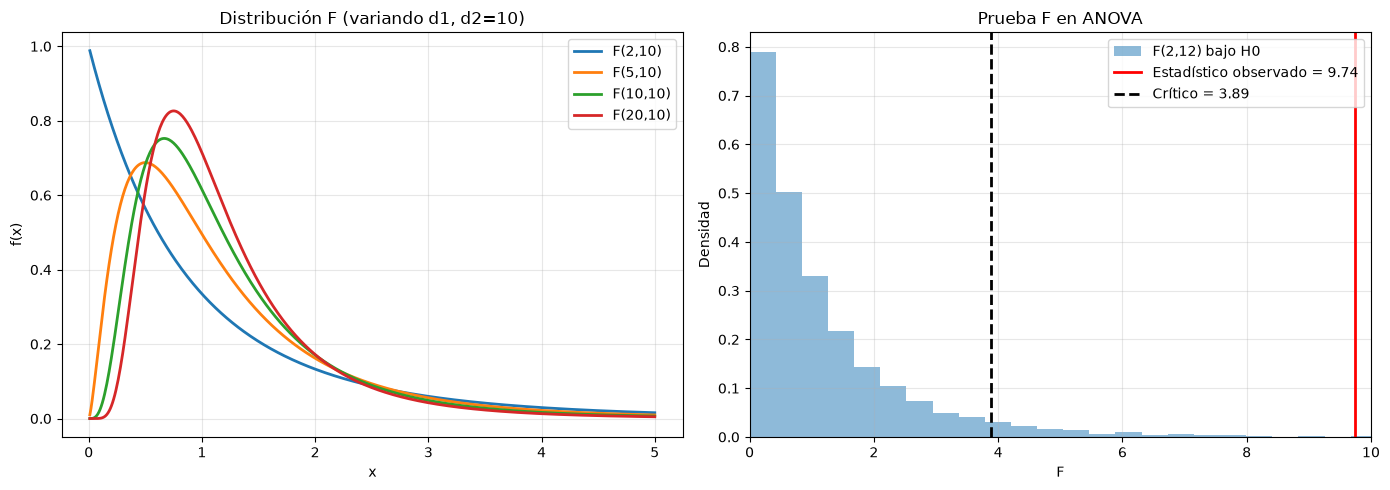
\includegraphics[height=7cm,keepaspectratio=true]{./pe/distF.png}
 % distF.png: 0x0 pixel, 300dpi, 0.00x0.00 cm, bb=
 \caption{Distribuci\'on $F$ de Snedecor y aplicaci\'on al ANOVA.}
 \label{fig:3.2.2}
\end{figure}



\subsection{Distribuciones de muestreo y ciencia de datos}

Las distribuciones de muestreo estudiadas en esta secci\'on son la base de las
t\'ecnicas m\'as usadas en ciencia de datos. A continuaci\'on se resumen las
aplicaciones principales.

\subsubsection{Tabla resumen}

\begin{center}
\begin{tabular}{|l|l|l|}
\hline
\textbf{Distribuci\'on} & \textbf{Estad\'istico} & \textbf{Aplicaci\'on} \\
\hline
$Z$ (normal est\'andar) & $\dfrac{\bar{X}-\mu}{\sigma/\sqrt{n}}$
& IC para $\mu$ con $\sigma$ conocida; prueba Z \\
\hline
$t$ de Student & $\dfrac{\bar{X}-\mu}{S/\sqrt{n}}$
& IC para $\mu$ con $\sigma$ desconocida; prueba t \\
\hline
$\chi^2$ & $\dfrac{(n-1)S^2}{\sigma^2}$
& IC para $\sigma^2$; prueba de bondad de ajuste \\
\hline
$F$ de Snedecor & $\dfrac{S_1^2}{S_2^2}$ o ANOVA
& Comparaci\'on de varianzas; ANOVA; F-test en regresi\'on \\
\hline
\end{tabular}
\end{center}

\subsubsection{Aplicaci\'on 1: A/B testing}

En A/B testing se comparan dos versiones de un producto midiendo alguna m\'etrica
de inter\'es (e.g., tasa de conversi\'on, tiempo en p\'agina).

\begin{ejemplo}
 \label{exmp:3.2.7}
Un sitio web tiene dos versiones: A (versi\'on actual) y B (nueva versi\'on). En
una prueba con $n_A = 1000$ usuarios de A, $x_A = 120$ convierten. En $n_B = 1000$
usuarios de B, $x_B = 145$ convierten. ¿Hay evidencia de que B es mejor?
\end{ejemplo}

\begin{solucion}
Estimamos las proporciones: $\hat{p}_A = 0.120$, $\hat{p}_B = 0.145$. Bajo la
hip\'otesis nula $H_0: p_A = p_B$, la proporci\'on agrupada es
\begin{align}
 \hat{p} = \frac{x_A + x_B}{n_A + n_B} = \frac{265}{2000} = 0.1325.
\end{align}
El error est\'andar agrupado es
\begin{align}
 \text{EE} = \sqrt{\hat{p}(1-\hat{p})\left(\frac{1}{n_A} + \frac{1}{n_B}\right)}
 = \sqrt{0.1325 \times 0.8675 \times 0.002} \approx 0.01516.
\end{align}
El estad\'istico $Z$ es
\begin{align}
 Z = \frac{\hat{p}_B - \hat{p}_A}{\text{EE}} = \frac{0.145 - 0.120}{0.01516} \approx 1.65.
\end{align}
Bajo $H_0$, $Z \sim N(0,1)$ aproximadamente. El $p$-valor bilateral es
$2(1 - \Phi(1.65)) \approx 0.099$. Al nivel $5\%$, no rechazamos $H_0$ (aunque al $10\%$
s\'i). El resultado es marginal.
\end{solucion}

[fragile, allowframebreaks]{abTesting.py}
 \begin{verbatim}
import numpy as np
from scipy import stats

# A/B testing
n_A, x_A = 1000, 120
n_B, x_B = 1000, 145
p_A = x_A / n_A
p_B = x_B / n_B
p_pool = (x_A + x_B) / (n_A + n_B)
se = np.sqrt(p_pool * (1 - p_pool) * (1/n_A + 1/n_B))
Z = (p_B - p_A) / se
p_valor = 2 * (1 - stats.norm.cdf(abs(Z)))
print(f"p_A = {p_A:.4f}, p_B = {p_B:.4f}")
print(f"Z = {Z:.3f}, p-valor = {p_valor:.4f}")
##p_A = 0.1200, p_B = 0.1450
##Z = 1.650, p-valor = 0.0989

# Bootstrap como alternativa no param\'etrica
np.random.seed(42)
boot_diffs = []
for _ in range(10000):
    boot_A = np.random.binomial(n_A, p_A) / n_A
    boot_B = np.random.binomial(n_B, p_B) / n_B
    boot_diffs.append(boot_B - boot_A)
ci = np.percentile(boot_diffs, [2.5, 97.5])
print(f"IC 95% bootstrap para p_B - p_A: [{ci[0]:.4f}, {ci[1]:.4f}]")
##IC 95% bootstrap para p_B - p_A: [-0.0002, 0.0498]
 \end{verbatim}

\subsubsection{Aplicaci\'on 2: Bootstrap}

El \emph{bootstrap} es una t\'ecnica no param\'etrica para estimar la distribuci\'on
muestral de un estad\'istico mediante remuestreo con reemplazo.

\begin{teorema}[Principio bootstrap]
Sea $X_1, \ldots, X_n$ una muestra iid de una distribuci\'on $F$ desconocida, y
$\theta = T(F)$ un par\'ametro de inter\'es. Si $\hat{\theta} = T(\hat{F}_n)$ es
el estimador plug-in (donde $\hat{F}_n$ es la distribuci\'on emp\'irica), entonces
la distribuci\'on muestral de $\hat{\theta}$ puede aproximarse por la distribuci\'on
de $\hat{\theta}^* = T(\hat{F}_n^*)$, donde $\hat{F}_n^*$ se obtiene al
remuestrear con reemplazo de la muestra original.
\end{teorema}

\begin{ejemplo}
 \label{exmp:3.2.8}
Considere una muestra de tama\~no $n = 50$ de una poblaci\'on con distribuci\'on
desconocida. Use bootstrap para estimar el sesgo y la varianza de la mediana
muestral.
\end{ejemplo}

\begin{solucion}
\begin{enumerate}
 \item Calcular la mediana observada $\hat{\theta} = \text{med}(X_1, \ldots, X_{50})$.
 \item Para $b = 1, \ldots, B$ (e.g., $B = 10000$):
   \begin{enumerate}
    \item Generar una muestra bootstrap $X_1^*, \ldots, X_{50}^*$ muestreando con
    reemplazo de la muestra original.
    \item Calcular la mediana bootstrap $\hat{\theta}_b^* = \text{med}(X_1^*, \ldots, X_{50}^*)$.
   \end{enumerate}
 \item Estimar:
   \begin{align}
    \widehat{\text{Sesgo}}_{\text{boot}} &= \frac{1}{B}\sum_{b=1}^B \hat{\theta}_b^* - \hat{\theta}, \\
    \widehat{\text{Var}}_{\text{boot}}(\hat{\theta}) &= \frac{1}{B-1}\sum_{b=1}^B (\hat{\theta}_b^* - \bar{\hat{\theta}}^*)^2.
   \end{align}
 \item El intervalo de confianza bootstrap al $95\%$ es
 $[\hat{\theta}_{\alpha/2}^*, \hat{\theta}_{1-\alpha/2}^*]$ donde los cuantiles
 se toman sobre $\{\hat{\theta}_b^*\}$.
\end{enumerate}
\end{solucion}

[fragile, allowframebreaks]{bootstrap.py}
 \begin{verbatim}
import numpy as np

# Simulaci\'on: poblaci\'on exponencial, estimamos la mediana
np.random.seed(42)
n = 50
poblacion = np.random.exponential(scale=2, size=10000)
muestra = np.random.exponential(scale=2, size=n)

# Mediana observada
theta_obs = np.median(muestra)
print(f"Mediana observada: {theta_obs:.3f}")
##Mediana observada: 1.485

# Bootstrap
B = 10000
thetas_boot = np.zeros(B)
for b in range(B):
    muestra_boot = np.random.choice(muestra, size=n, replace=True)
    thetas_boot[b] = np.median(muestra_boot)

# Estimaciones bootstrap
sesgo = np.mean(thetas_boot) - theta_obs
var = np.var(thetas_boot, ddof=1)
print(f"Sesgo bootstrap: {sesgo:.3f}")
print(f"Varianza bootstrap: {var:.4f}")
##Sesgo bootstrap: 0.029
##Varianza bootstrap: 0.0707

# IC al 95\% (m\'etodo percentil)
ic = np.percentile(thetas_boot, [2.5, 97.5])
print(f"IC 95% bootstrap: [{ic[0]:.3f}, {ic[1]:.3f}]")
##IC 95% bootstrap: [0.971, 2.025]
 \end{verbatim}

\subsubsection{Aplicaci\'on 3: Inferencia en Machine Learning}

En machine learning, las distribuciones de muestreo subyacen a:

\begin{itemize}
 \item \textbf{Validaci\'on cruzada}: la varianza del estimador de error de
 generalizaci\'on se puede estimar mediante bootstrap o mediante la distribuci\'on
 $t$ (con n\'umero de folds como grados de libertad).
 \item \textbf{Pruebas de hip\'otesis para comparar modelos}: se usan pruebas
 $t$ pareadas para comparar dos modelos en los mismos datos, o pruebas $F$ para
 comparar modelos anidados (e.g., regresi\'on lineal).
 \item \textbf{Intervalos de confianza para m\'etricas}: precisi\'on y recall
 tienen distribuciones aproximadamente normales para muestras grandes; su IC
 se construye con $Z$ o $t$.
 \item \emph{Feature selection}: el test $F$ se usa para evaluar la significancia
 global de un modelo de regresi\'on, y los tests $\chi^2$ para evaluar
 independencia entre variables.
\end{itemize}

\begin{observacion}
En deep learning, las distribuciones de muestreo son menos prominentes porque los
modelos se entrenan con grandes vol\'umenes de datos y se eval\'uan con conjuntos
de prueba, no con pruebas de hip\'otesis cl\'asicas. Sin embargo, siguen siendo
fundamentales para:
\begin{itemize}
 \item Comparar arquitecturas mediante pruebas de hip\'otesis sobre m\'etricas de
 rendimiento agregadas.
 \item Estimar la incertidumbre de las predicciones (intervalos de confianza,
 predicci\'on conformal).
 \item Cuantificar la significancia estad\'istica de mejoras en benchmarks.
\end{itemize}
\end{observacion}



